\documentclass{beamer}
%
% Choose how your presentation looks.
%
% For more themes, color themes and font themes, see:
% http://deic.uab.es/~iblanes/beamer_gallery/index_by_theme.html
%
\mode<presentation>
{
  \usetheme{default}      % or try Darmstadt, Madrid, Warsaw, ...
  \usecolortheme{default} % or try albatross, beaver, crane, ...
  \usefonttheme{default}  % or try serif, structurebold, ...
  \setbeamertemplate{navigation symbols}{}
  \setbeamertemplate{caption}[numbered]
} 

\usepackage[english]{babel}
\usepackage[utf8]{inputenc}
\usepackage[T1]{fontenc}
\usepackage{bm, colonequals, xcolor}


\newcommand{\bh}{\mathbf{h}}
\newcommand{\bu}{\mathbf{u}}
\newcommand{\bl}{\mathbf{l}}
\newcommand{\ba}{\mathbf{a}}
\newcommand{\bv}{\mathbf{v}}
\newcommand{\bc}{\mathbf{c}}
\newcommand{\bb}{\mathbf{b}}
\newcommand{\bs}{\mathbf{s}}
\newcommand{\bp}{\mathbf{p}}
\newcommand{\bx}{\mathbf{x}}
\newcommand{\by}{\mathbf{y}}
\newcommand{\bq}{\mathbf{q}}
\newcommand{\bg}{\mathbf{g}}
\newcommand{\bk}{\mathbf{k}}
\newcommand{\br}{\mathbf{r}}
\newcommand{\bw}{\mathbf{w}}
\newcommand{\bS}{\mathbf{S}}
\newcommand{\bT}{\mathbf{T}}
\newcommand{\bz}{\mathbf{z}}
\newcommand{\bZ}{\mathbf{Z}}
\newcommand{\bO}{\mathbf{O}}
\newcommand{\bP}{\mathbf{P}}
\newcommand{\bA}{\mathbf{A}}
\newcommand{\bY}{\mathbf{Y}}
\newcommand{\bJ}{\mathbf{J}}
\newcommand{\bW}{\mathbf{W}}
\newcommand{\bF}{\mathbf{F}}
\newcommand{\bG}{\mathbf{G}}
\newcommand{\bE}{\mathbf{E}}
\newcommand{\bL}{\mathbf{L}}
\newcommand{\bN}{\mathbf{N}}
\newcommand{\bI}{\mathbf{I}}
\newcommand{\bD}{\mathbf{D}}
\newcommand{\bH}{\mathbf{H}}
\newcommand{\bU}{\mathbf{U}}
\newcommand{\bV}{\mathbf{V}}
\newcommand{\bK}{\mathbf{K}}
\newcommand{\bX}{\mathbf{X}}
\newcommand{\bQ}{\mathbf{Q}}
\newcommand{\bB}{\mathbf{B}}
\newcommand{\bC}{\mathbf{C}}
\newcommand{\bM}{\mathbf{M}}
\newcommand{\bR}{\mathbf{R}}


\newcommand{\bfzero}{\mathbf{0}}
\newcommand{\bfalpha}{\bm{\alpha}}
\newcommand{\bfgamma}{\bm{\gamma}}
\newcommand{\bfmu}{\bm{\mu}}
\newcommand{\bfxi}{\bm{\xi}}
\newcommand{\bftheta}{\bm{\theta}}
\newcommand{\bfeta}{\bm{\eta}}
\newcommand{\bfnu}{\bm{\nu}}
\newcommand{\bfdelta}{\bm{\delta}}
\newcommand{\bfkappa}{\bm{\kappa}}
\newcommand{\bfbeta}{\bm{\beta}}
\newcommand{\bfepsilon}{\bm{\epsilon}}
\newcommand{\bftau}{\bm{\tau}}
\newcommand{\bfomega}{\bm{\omega}}
\newcommand{\bfpi}{\bm{\pi}}
\newcommand{\bfpsi}{\bm{\psi}}
\newcommand{\bfrho}{\bm{\rho}}
\newcommand{\bfSigma}{\bm{\Sigma}}
\newcommand{\bfGamma}{\bm{\Gamma}}
\newcommand{\bfLambda}{\bm{\Lambda}}
\newcommand{\bfPsi}{\bm{\Psi}}
\newcommand{\bfOmega}{\bm{\Omega}}
\newcommand{\blt}{\tilde{\bL}}

\newcommand{\normal}{\mathcal{N}}
\newcommand{\grid}{\mathcal{G}}
\newcommand{\var}{\textbf{Var}}



\title[Linear Vecchia filtering]{Vecchia filters for linear models with Gaussian data}
\author{Marcin Jurek}
\institute{Texas A\&M}
\date{May 12, 2020}

\begin{document}

\begin{frame}
  \titlepage
\end{frame}

% Uncomment these lines for an automatically generated outline.
%\begin{frame}{Outline}
%  \tableofcontents
%\end{frame}

\section{Overview}

\begin{frame}{The problem}
    Let $\bx_t$ be the discretized values at time $t$ of the Gaussian process we are interested in.
    
    \vspace{1cm}
    Using domain knowledge, we also know that
    $$
    \bx_t = \mathcal{E}_t(\bx_{t-1}) + \bw_t, \quad\quad \text{where } \bw_t \sim \mathcal{N}(\bfzero, \bQ_t).
    $$
    where $\mathcal{E}_t$ is some function, possibly non-linear.
    
\end{frame}

\begin{frame}{The problem}


But we don't observe $\bx_t$. Instead, we have
$$
\by_t = \bH_t\bx_t + \bv_t, \quad\quad \text{where } \bv_t \sim \mathcal{N}(\bfzero, \bR_t).
$$
Note that here we assume Gaussian measurement error. This is not necessary in the strict sense, but we will focus on this case for now. The more general case is about to be published.

\vspace{1cm}
We want to infer the \emph{filtering distribtution}, i.e.
$$
\bx_t | \by_{1:t} 
$$

\end{frame}



\begin{frame}{Traditional methods}
When the temporal evolution operator ($\mathcal{E}_t$) is linear (i.e. $\mathcal{E}_t(\bx_{t-1}) = \bE_t\bx_{t-1})$ we normally use the Kalman filter:

Assuming that at time $t=0$ we have 
$$\bx_0 \sim \normal(\bfmu_{0|0}, \bfSigma_{0|0})$$
\textbf{Forecast step:}
\begin{itemize}
    \item Calculate $\bfmu_{t|t-1} = \bE_t \bfmu_{t|t}$
    \item Calculate $\bfSigma_{t|t-1} = \bE_t \bfSigma_{t-1|t-1} \bE_t' + \bQ_t$.
\end{itemize}
\textbf{Update step:}
\begin{itemize}
    \item Calculate $\bK_t \colonequals \bfSigma_{t|t-1}\bH_t'\color{red}(\bH_t\bfSigma_{t|t-1} \bH_t'+\bR_t)^{-1}$
    \item Calculate $\bfmu_{t|t} \colonequals \bfmu_{t|t-1} + \bK_t(\by_t - \bH_t \bfmu_{t|t-1})$
    \item Calculate $\bfSigma_{t|t} \colonequals (\bI_{n_\grid} - \bK_t \bH_t) \bfSigma_{t|t-1}$
\end{itemize}
\end{frame}


\begin{frame}{Traditional methods}
    Some other methods
    \begin{itemize}
        \item low-rank filters (LR)
        \item Ensemble Kalman filter (EnKF)
        \item filtering in the spectral domain
    \end{itemize}

\vspace{0.5cm}
But: EnKF is using only an ensemble to represent the entire distribution, low-rank filter, is, well... low-rank and (as far as I know) you can do filtering in the spectral domain only in some very special cases.

\vspace{0.5cm}
There are so many spatial approximations, what's the problem?
\end{frame}

\begin{frame}{Multi-resolution approximation}
    A special basis of functions with decreasing (and "nested") support.
    \begin{figure}
        \centering
        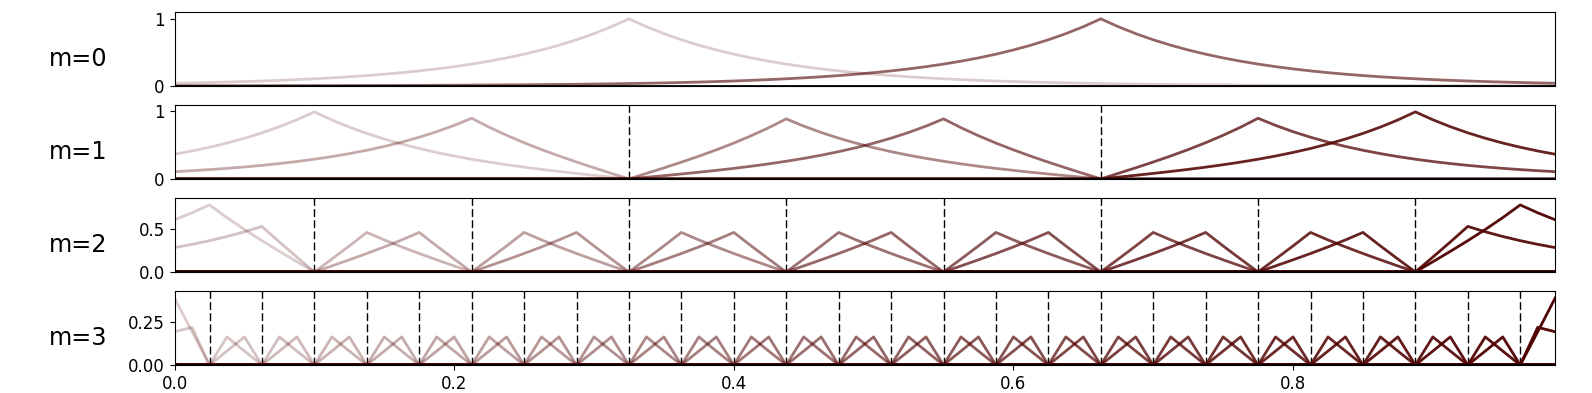
\includegraphics[width=1.0\textwidth]{plots/basisf-prior.png}
    \end{figure}
    \vfill
    In terms of matrix approximations
    \begin{figure}
        \centering
        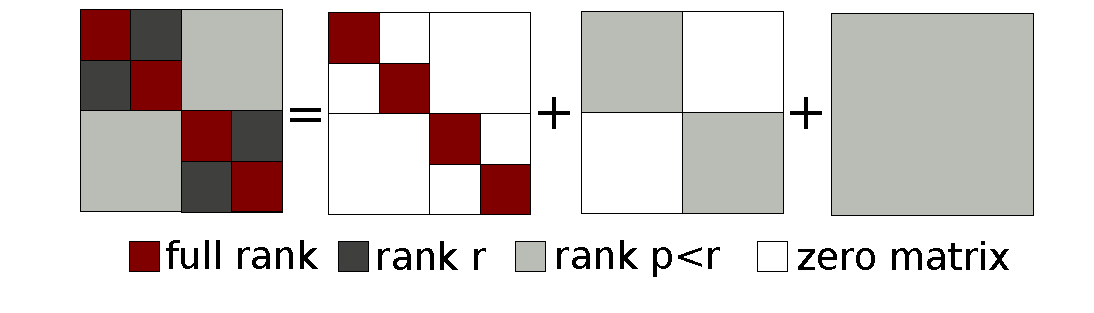
\includegraphics[width=0.85\textwidth]{plots/2LHODLRsum.pdf}
    \end{figure}
\end{frame}


\begin{frame}{MRA as Vecchia}
\begin{figure}
        \centering
        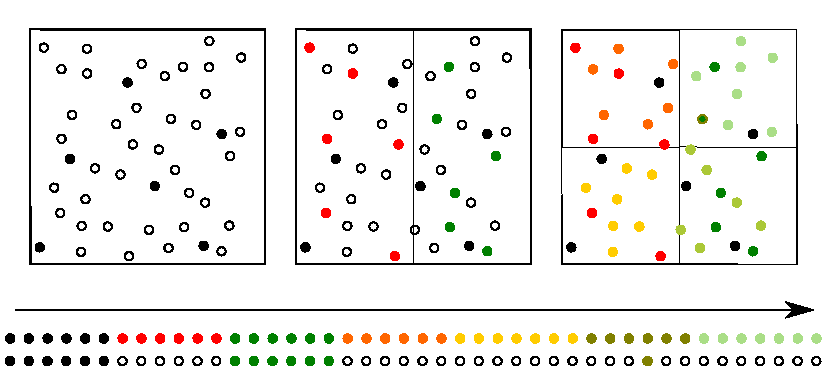
\includegraphics[width=\textwidth]{plots/domain.pdf}
\end{figure}
\end{frame}


\begin{frame}{Why is the MRA good for filtering?}
    Using the basis function approach, MRA enables us to write:
    $$
    \bx_t = \bB_t \eta_t, \quad \text{where } \eta_t \sim \normal(0, \bI)
    $$
    where $\bB_t$ has this special pattern corresponding to the support of each function in the MRA family:
    \begin{figure}
        \centering
        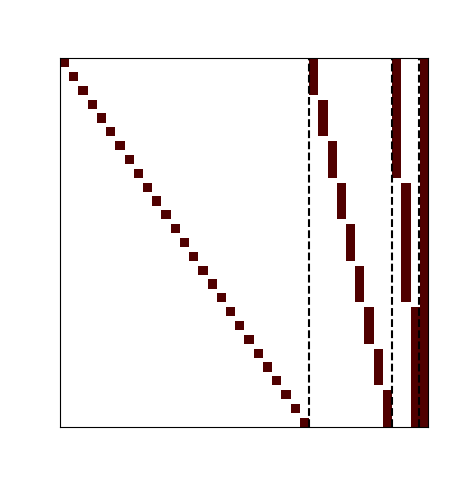
\includegraphics[width=0.5\textwidth]{plots/B.png}
    \end{figure}
\end{frame}


\begin{frame}{Why is the MRA good for filtering?}
    What is so special about this structure? Recall the bottleneck in the Kalman filter:
    $$
    (\bH_t\bfSigma_{t|t-1} \bH_t'+\bR_t)^{-1}
    $$
    If we approximate $\bx_t \approx \bB_t\bfeta_t$ then, in particular $\var(\bx_t) \approx \bB_t\bB_t'$ and (dropping time subscripts)
    \begin{multline*}
    (\bH\bfSigma_{t|t-1} \bH'+\bR)^{-1} \approx (\bH\bB\bB \bH'+\bR)^{-1} = \\
    \bR^{-1} + \bR^{-1}\bH\bB(\bI + \bH'\bB'\bR\bB\bH)^{-1}\bB'\bH'\bR_t^{-1} \\ \approx 
    \bI + \bB(\bI + \bB'\bB)^{-1}\bB' \equalscolon\bfLambda
    \end{multline*}
\end{frame}

\begin{frame}{Why is the MRA good for filtering}
    If you do the math and define $\bL = \text{chol}(\bfLambda)$ then 
    $$
    \bfSigma_{t|t} = \bB\bfLambda\bB' = \bB\bL\bL'\bB' 
    $$
    Amazingly, $\tilde{\bB} \colonequals \bB\bL$, has the same sparsity pattern as $\bB$.
    
    \vspace{1cm}
    This means, instead of work with $\bB$s instead of $\bfSigma_{t|t}$s.
    \vfill
    Let's see how it changes the filtering algo.
\end{frame}



\begin{frame}{Vecchia filter}
Assuming that at time $t=0$ we have 
$$\bx_0 \sim \normal(\bfmu_{0|0}, \bfSigma_{0|0})$$
\textbf{Forecast step:}
\begin{itemize}
    \item Calculate $\bfmu_{t|t-1} = \bE_t \bfmu_{t|t}$
    \item Calculate $\bfSigma_{t|t-1} = \bE_t \bfSigma_{t-1|t-1} \bE_t' + \bQ_t$.
\end{itemize}
\textbf{Update step:}
\begin{itemize}
    \item Calculate $\bK_t \colonequals \bfSigma_{t|t-1}\bH_t'(\bH_t\bfSigma_{t|t-1} \bH_t'+\bR_t)^{-1}$
    \item Calculate $\bfmu_{t|t} \colonequals \bfmu_{t|t-1} + \bK_t(\by_t - \bH_t \bfmu_{t|t-1})$
    \item Calculate $\bfSigma_{t|t} \colonequals (\bI_{n_\grid} - \bK_t \bH_t) \bfSigma_{t|t-1}$
\end{itemize}
\end{frame}



\begin{frame}{Vecchia filter}
Assuming that at time $t=0$ we have 
$$\bx_0 \sim \normal(\bfmu_{0|0}, \color{red}\bB_{0|0}\bB_{0|0}'\color{black})$$
\textbf{Forecast step:}
\begin{itemize}
    \item Calculate $\bfmu_{t|t-1} = \bE_t \bfmu_{t|t}$
    \item Calculate $\bfSigma_{t|t-1} = \bE_t \bfSigma_{t-1|t-1} \bE_t' + \bQ_t$.
\end{itemize}
\textbf{Update step:}
\begin{itemize}
    \item Calculate $\bK_t \colonequals \bfSigma_{t|t-1}\bH_t'(\bH_t\bfSigma_{t|t-1} \bH_t'+\bR_t)^{-1}$
    \item Calculate $\bfmu_{t|t} \colonequals \bfmu_{t|t-1} + \bK_t(\by_t - \bH_t \bfmu_{t|t-1})$
    \item Calculate $\bfSigma_{t|t} \colonequals (\bI_{n_\grid} - \bK_t \bH_t) \bfSigma_{t|t-1}$
\end{itemize}
\end{frame}



\begin{frame}{Vecchia filter}
Assuming that at time $t=0$ we have 
$$\bx_0 \sim \normal(\bfmu_{0|0}, \bB_{0|0}\bB_{0|0}')$$
\textbf{Forecast step:}
\begin{itemize}
    \item Calculate $\bfmu_{t|t-1} = \bE_t \bfmu_{t|t}$
    \item Calculate \color{red}$\bB_{t|t-1} s.t. \newline \bB_{t|t-1} \bB'_{t|t-1} = \bE_t \bfSigma_{t-1|t-1} \bE_t' + \bQ_t$.
\end{itemize}
\textbf{Update step:}
\begin{itemize}
    \item Calculate $\bK_t \colonequals \bfSigma_{t|t-1}\bH_t'(\bH_t\bfSigma_{t|t-1} \bH_t'+\bR_t)^{-1}$
    \item Calculate $\bfmu_{t|t} \colonequals \bfmu_{t|t-1} + \bK_t(\by_t - \bH_t \bfmu_{t|t-1})$
    \item Calculate $\bfSigma_{t|t} \colonequals (\bI_{n_\grid} - \bK_t \bH_t) \bfSigma_{t|t-1}$
\end{itemize}
\end{frame}


\begin{frame}{Vecchia filter}
Assuming that at time $t=0$ we have 
$$\bx_0 \sim \normal(\bfmu_{0|0}, \bB_{0|0}\bB_{0|0}')$$
\textbf{Forecast step:}
\begin{itemize}
    \item Calculate $\bfmu_{t|t-1} = \bE_t \bfmu_{t|t}$
    \item Calculate $\bB_{t|t-1} s.t. \newline \bB_{t|t-1} \bB'_{t|t-1} = \bE_t \bfSigma_{t-1|t-1} \bE_t' + \bQ_t$.
\end{itemize}
\textbf{Update step:}
\begin{itemize}
    \item Calculate \color{red}$\bfLambda \colonequals (\bI + \bB_{t|t-1}'\bH_t'\bR_t^{-1}\bH_t\bB_{t|t-1})^{-1}$\color{black}.
    \item Calculate $\bfmu_{t|t} \colonequals \bfmu_{t|t-1} + \bK_t(\by_t - \bH_t \bfmu_{t|t-1})$
    \item Calculate $\bfSigma_{t|t} \colonequals (\bI_{n_\grid} - \bK_t \bH_t) \bfSigma_{t|t-1}$
\end{itemize}
\end{frame}


\begin{frame}{Vecchia filter}
Assuming that at time $t=0$ we have 
$$\bx_0 \sim \normal(\bfmu_{0|0}, \bB_{0|0}\bB_{0|0}')$$
\textbf{Forecast step:}
\begin{itemize}
    \item Calculate $\bfmu_{t|t-1} = \bE_t \bfmu_{t|t}$
    \item Calculate $\bB_{t|t-1} s.t. \newline \bB_{t|t-1} \bB'_{t|t-1} = \bE_t \bfSigma_{t-1|t-1} \bE_t' + \bQ_t$.
\end{itemize}
\textbf{Update step:}
\begin{itemize}
    \item Calculate $\bfLambda \colonequals (\bI + \bB_{t|t-1}'\bH_t'\bR_t^{-1}\bH_t\bB_{t|t-1})^{-1}$.
    \item Calculate $\color{red}\bB_{t|t} \colonequals \bB_{t|t}\text{chol}(\bfLambda_t)\color{black}$
    \item Calculate $\bfmu_{t|t} \colonequals \bfmu_{t|t-1} + \bK_t(\by_t - \bH_t \bfmu_{t|t-1})$
    \item Calculate $\bfSigma_{t|t} \colonequals (\bI_{n_\grid} - \bK_t \bH_t) \bfSigma_{t|t-1}$
\end{itemize}
\end{frame}



\begin{frame}{Vecchia filter}
Assuming that at time $t=0$ we have 
$$\bx_0 \sim \normal(\bfmu_{0|0}, \bB_{0|0}\bB_{0|0}')$$
\textbf{Forecast step:}
\begin{itemize}
    \item Calculate $\bfmu_{t|t-1} = \bE_t \bfmu_{t|t}$
    \item Calculate $\bB_{t|t-1} s.t. \newline \bB_{t|t-1} \bB'_{t|t-1} = \bE_t \bfSigma_{t-1|t-1} \bE_t' + \bQ_t$.
\end{itemize}
\textbf{Update step:}
\begin{itemize}
    \item Calculate $\bfLambda \colonequals (\bI + \bB_{t|t-1}'\bH_t'\bR_t^{-1}\bH_t\bB_{t|t-1})^{-1}$.
    \item Calculate $\bB_{t|t} \colonequals \bB_{t|t}\text{chol}(\bfLambda_t)$
    \item Calculate $\bfmu_{t|t} \colonequals \bfmu_{t|t-1} +\color{red}\bB_{t|t}\bB_{t|t}'\bH_t'\bR_t^{-1}\color{black}(\by_t - \bH_t \bfmu_{t|t-1})$
    \item Calculate $\bfSigma_{t|t} \colonequals (\bI_{n_\grid} - \bK_t \bH_t) \bfSigma_{t|t-1}$
\end{itemize}
\end{frame}



\begin{frame}{Vecchia filter}
Assuming that at time $t=0$ we have 
$$\bx_0 \sim \normal(\bfmu_{0|0}, \bB_{0|0}\bB_{0|0}')$$
\textbf{Forecast step:}
\begin{itemize}
    \item Calculate $\bfmu_{t|t-1} = \bE_t \bfmu_{t|t}$
    \item Calculate $\bB_{t|t-1} s.t. \newline \bB_{t|t-1} \bB'_{t|t-1} = \bE_t \bfSigma_{t-1|t-1} \bE_t' + \bQ_t$.
\end{itemize}
\textbf{Update step:}
\begin{itemize}
    \item Calculate $\bfLambda \colonequals (\bI + \bB_{t|t-1}'\bH_t'\bR_t^{-1}\bH_t\bB_{t|t-1})^{-1}$.
    \item Calculate $\bB_{t|t} \colonequals \bB_{t|t}\text{chol}(\bfLambda_t)$
    \item Calculate $\bfmu_{t|t} \colonequals \bfmu_{t|t-1} +\bB_{t|t}\bB_{t|t}'\bH_t'\bR_t^{-1}(\by_t - \bH_t \bfmu_{t|t-1})$\color{red}
    \item (x)
\end{itemize}
\end{frame}



\begin{frame}{Vecchia filter}
Assuming that at time $t=0$ we have 
$$\bx_0 \sim \normal(\bfmu_{0|0}, \bB_{0|0}\bB_{0|0}')$$
\textbf{Forecast step:}
\begin{itemize}
    \item Calculate $\bfmu_{t|t-1} = \bE_t \bfmu_{t|t}$
    \item Calculate $\bB_{t|t-1} s.t. \newline \bB_{t|t-1} \bB'_{t|t-1} = \bE_t \bfSigma_{t-1|t-1} \bE_t' + \bQ_t$.
\end{itemize}
\textbf{Update step:}
\begin{itemize}
    \item Calculate $\bfLambda \colonequals (\bI + \bB_{t|t-1}'\bH_t'\bR_t^{-1}\bH_t\bB_{t|t-1})^{-1}$.
    \item Calculate $\bB_{t|t} \colonequals \bB_{t|t}\text{chol}(\bfLambda_t)$
    \item Calculate $\bfmu_{t|t} \colonequals \bfmu_{t|t-1} +\bB_{t|t}\bB_{t|t}'\bH_t'\bR_t^{-1}(\by_t - \bH_t \bfmu_{t|t-1})$\color{red}
\end{itemize}
\end{frame}



\begin{frame}{Why this works}

So as you can see it all hinges on the fact that 
$$\bB_{t|t} = \bB_{t|t}\text{chol}(\bfLambda_t)$$
has the same sparsity as $\bB_{t|t-1}$ and $\bB_{t-1|t-1}$. This is how it looks like:
\begin{figure}
\centering
			\begin{figure}
				\centering
				\begin{tabular}{ccc}
				\raisebox{-.5\height}{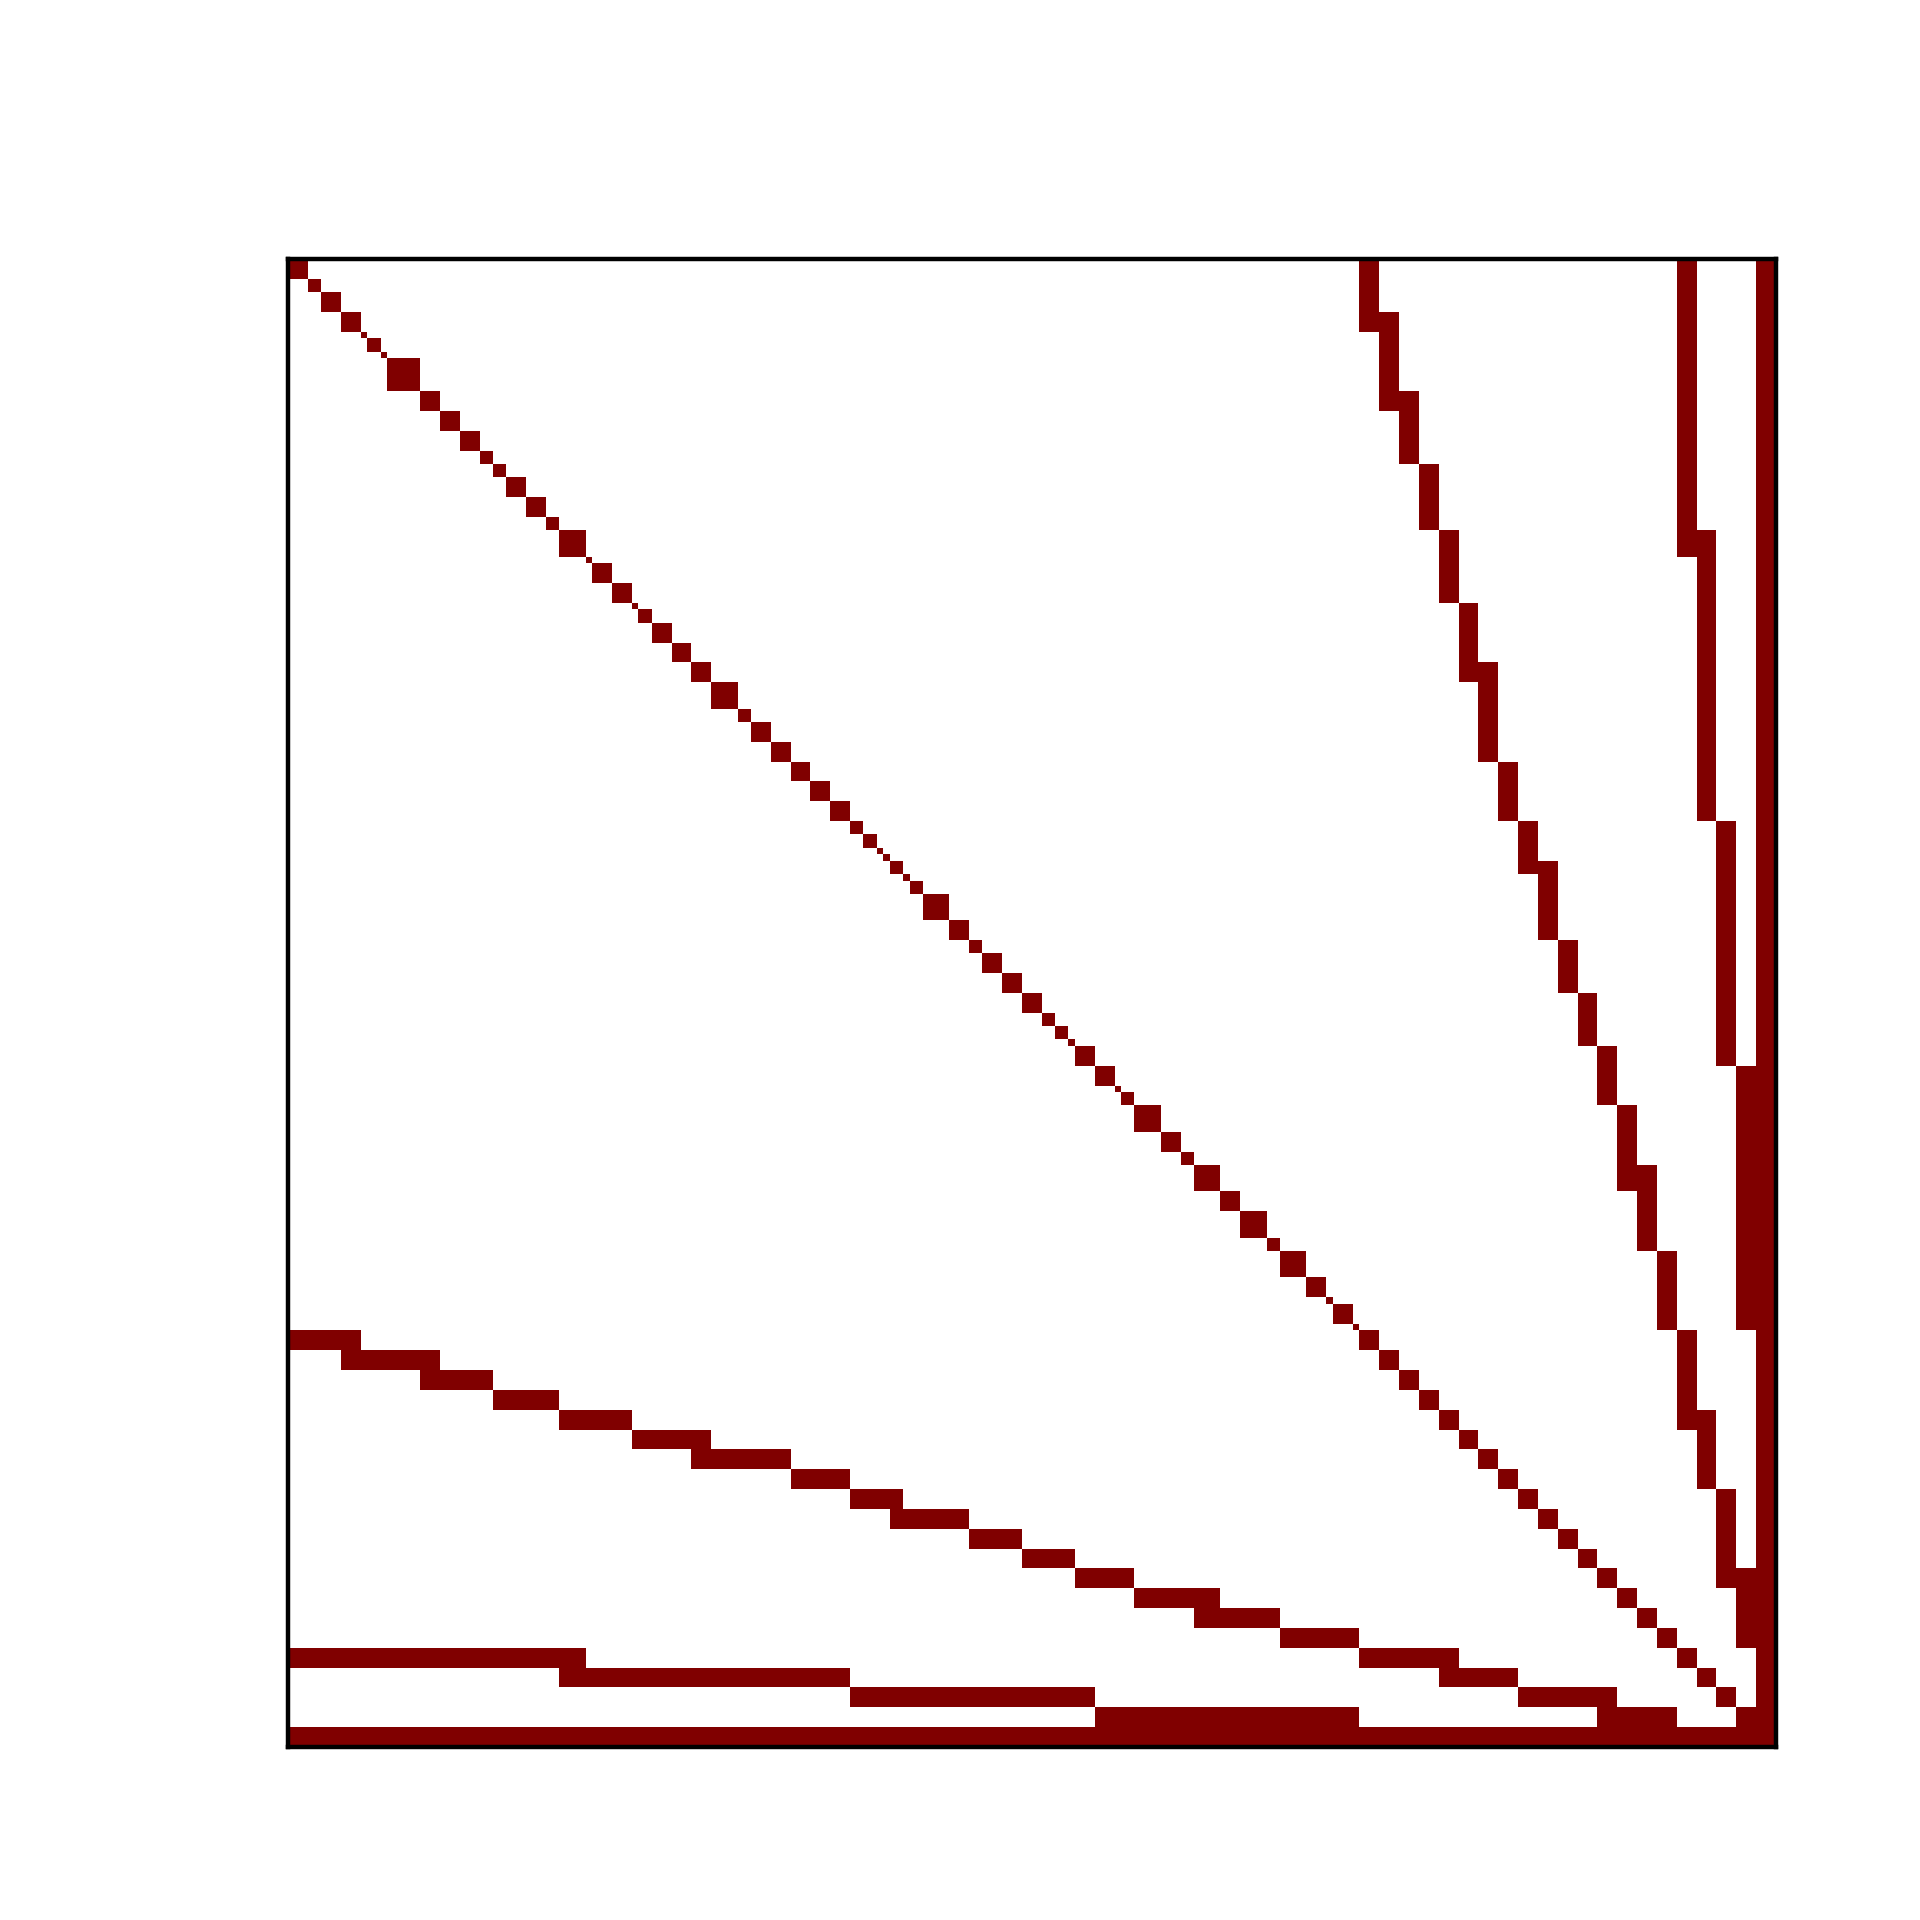
\includegraphics[scale=0.26]{plots/BB.png}} &  \raisebox{-.5\height}{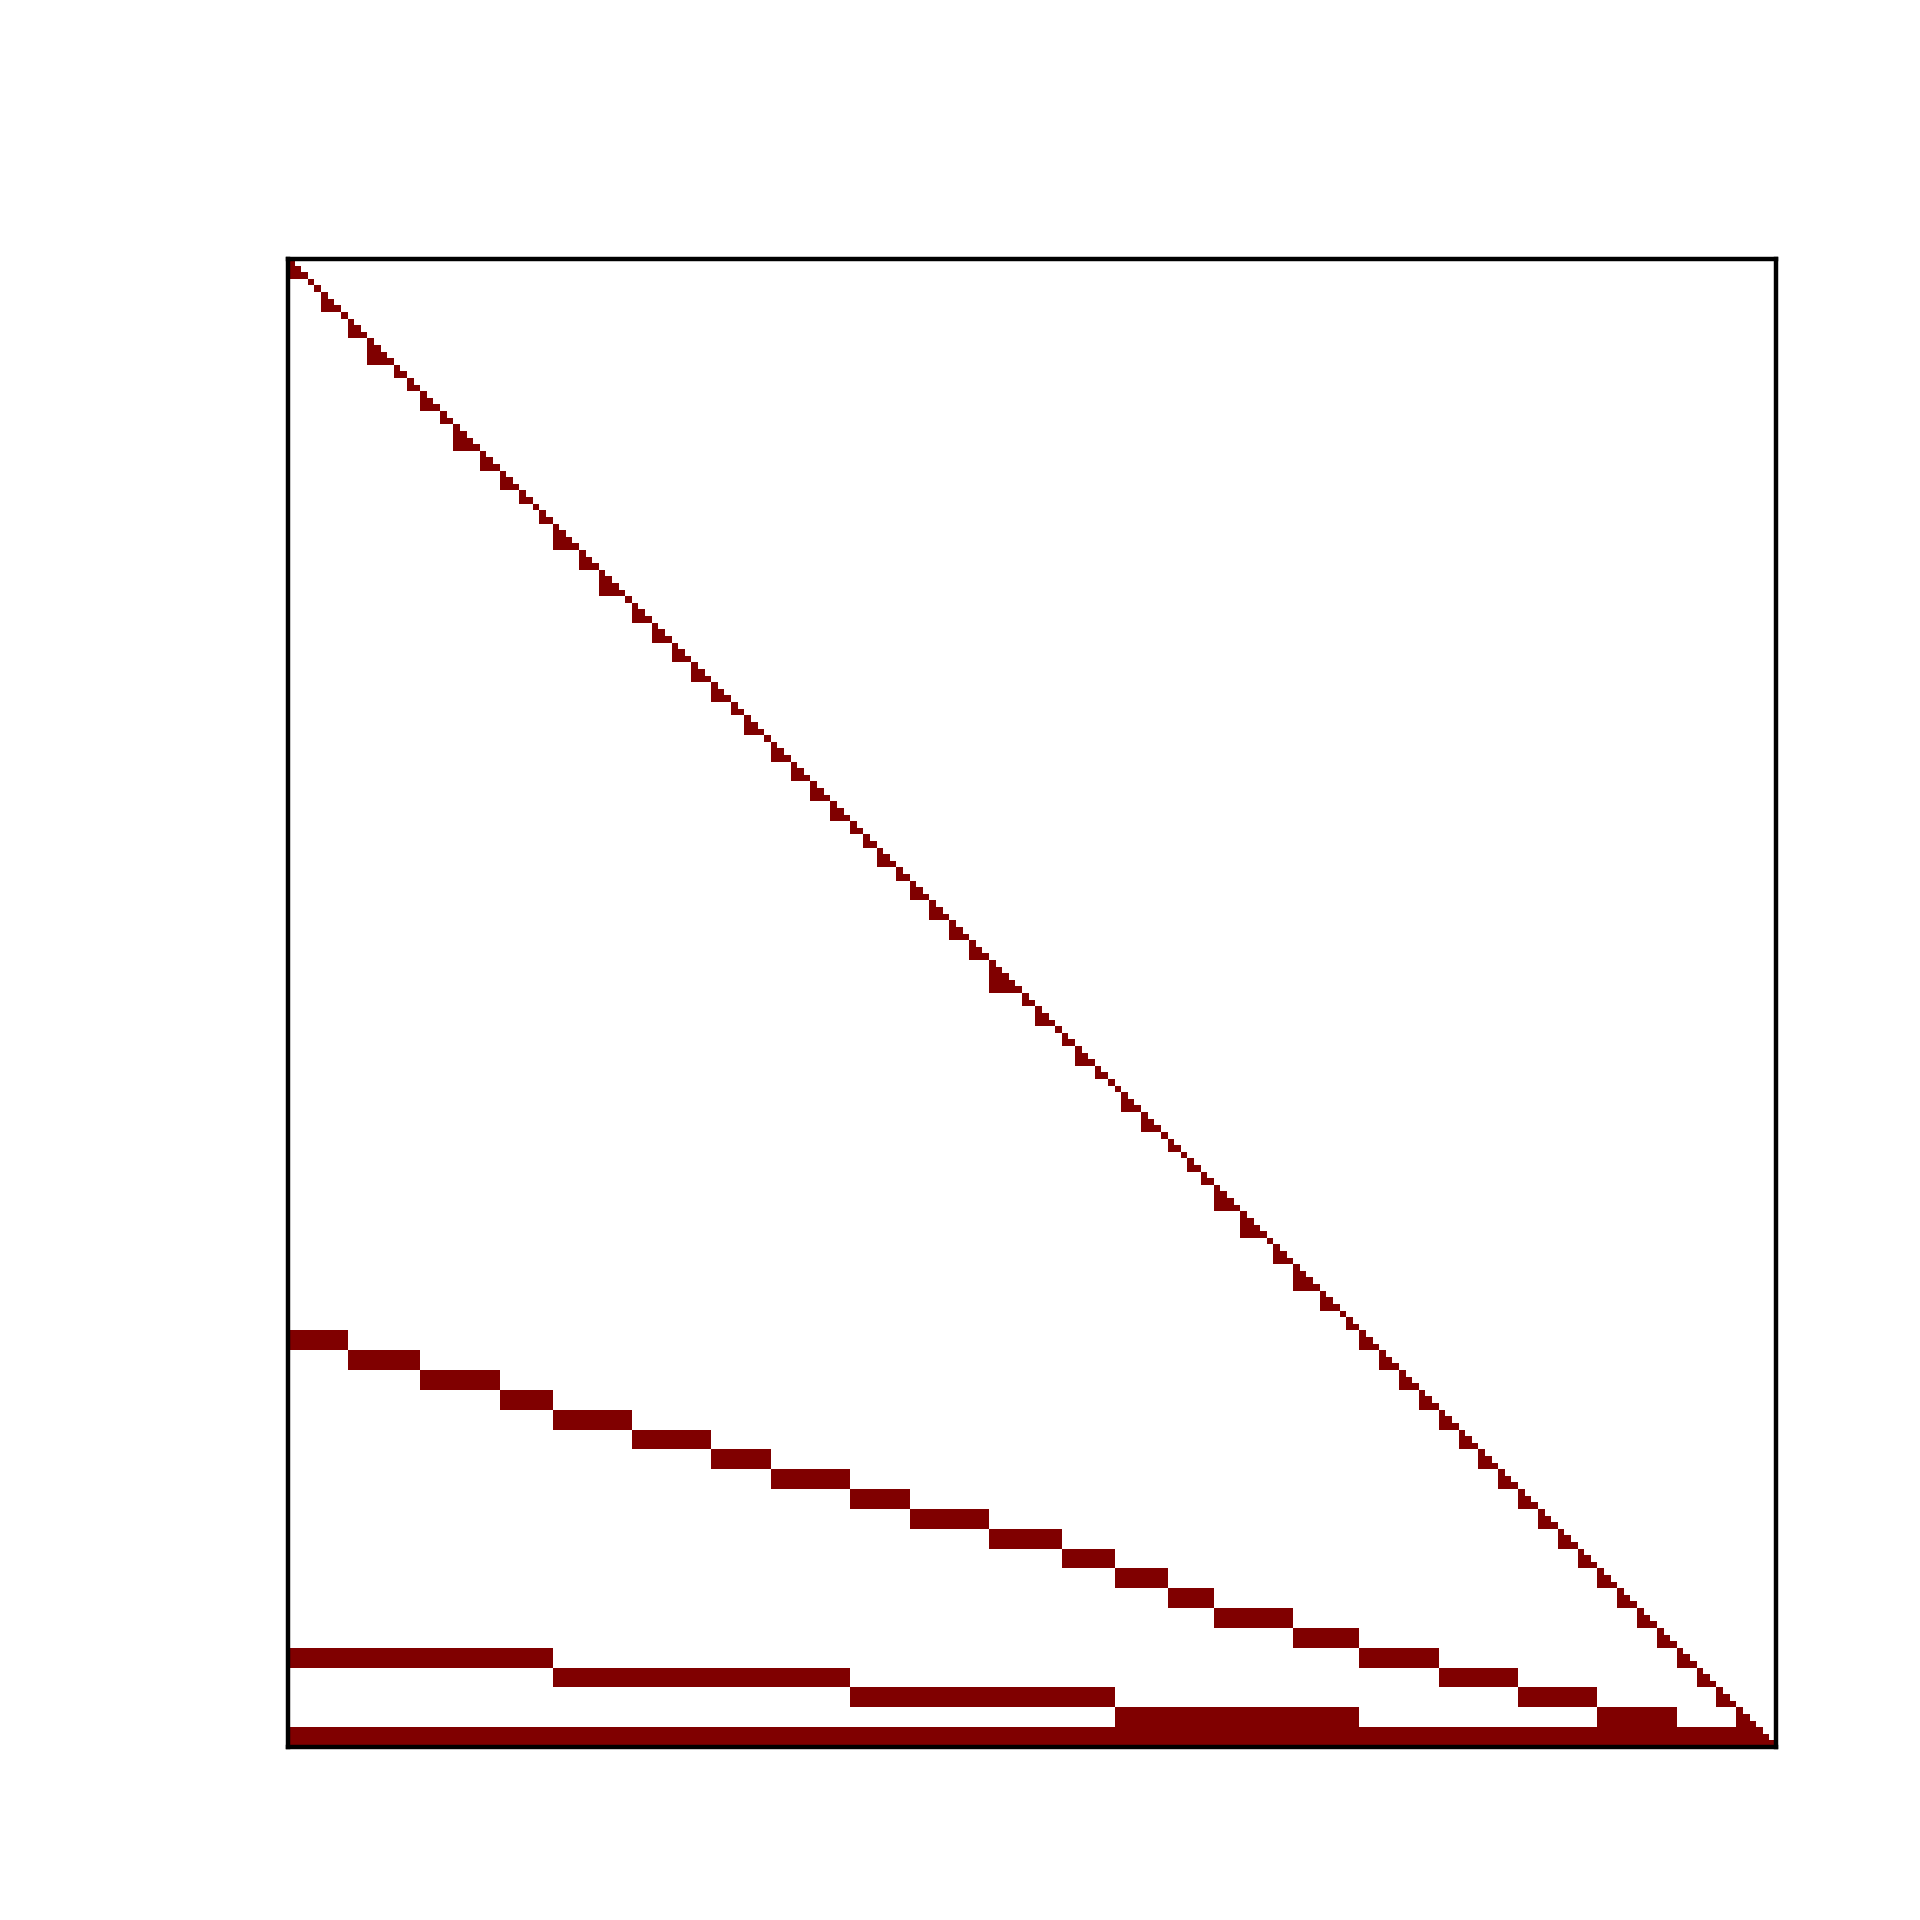
\includegraphics[scale=0.26]{plots/BTBc.png}} & \raisebox{-.5\height}{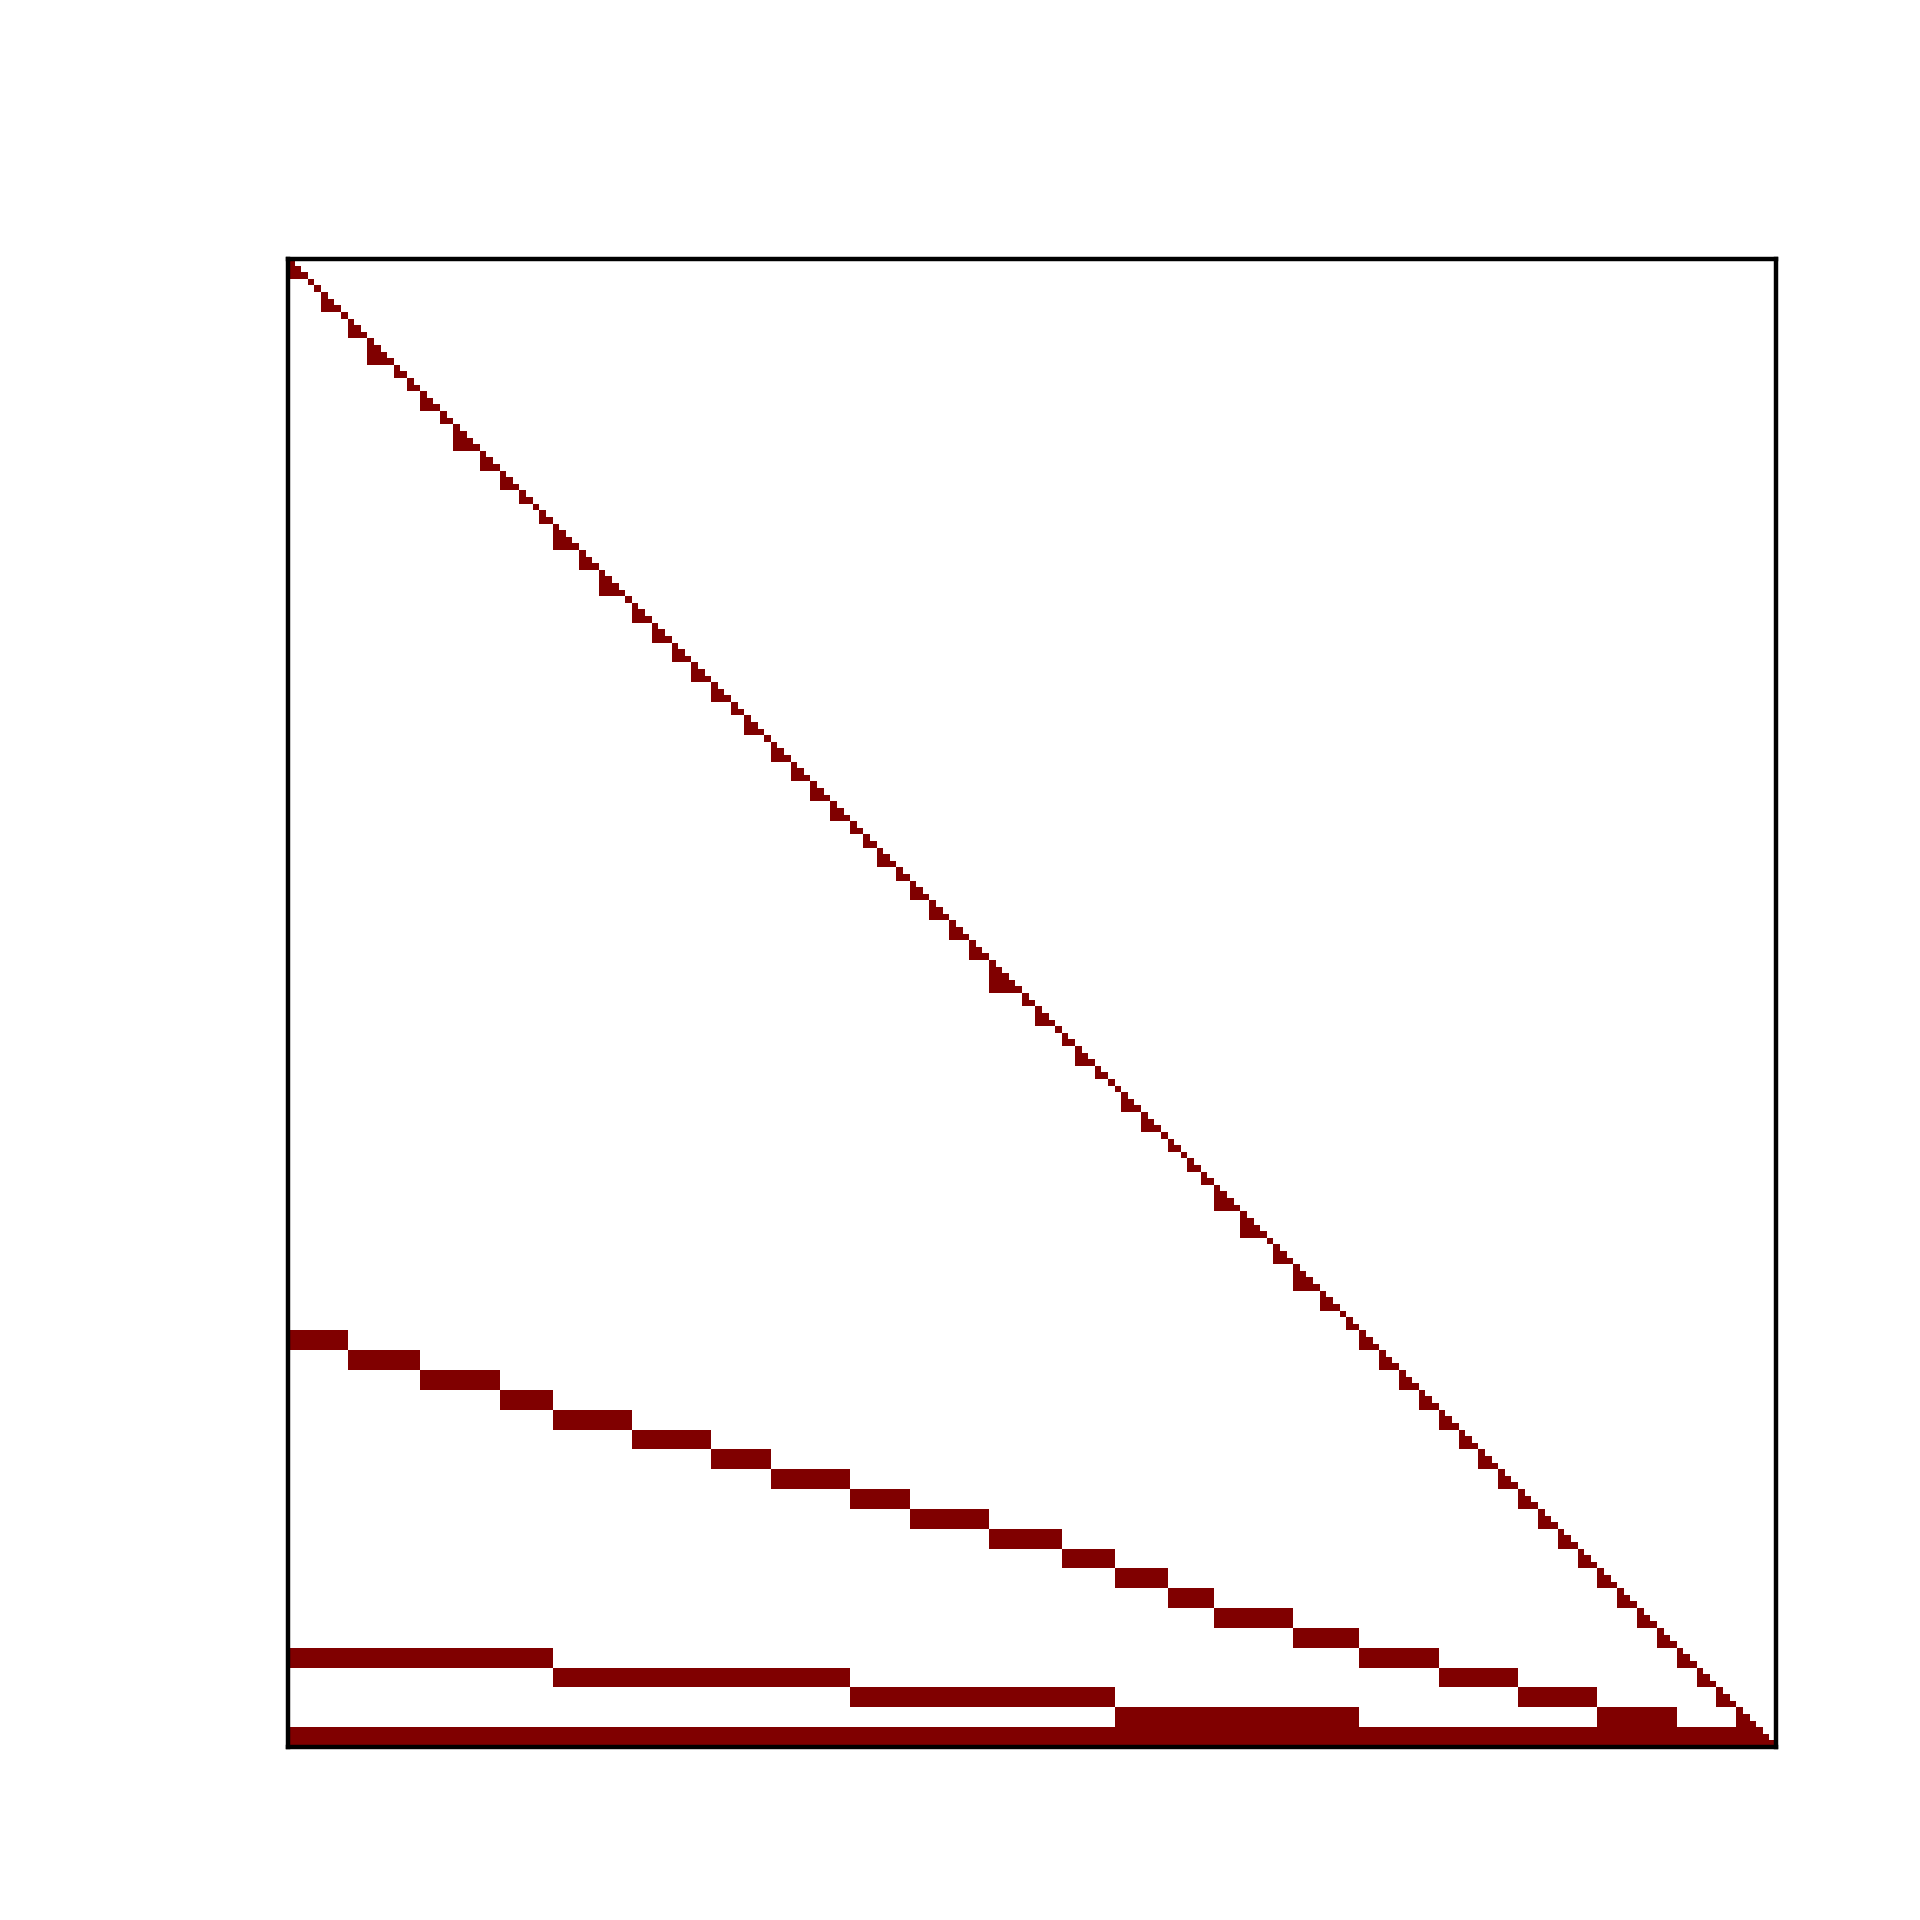
\includegraphics[scale=0.26]{plots/BTBcInv.png}} \\
				$\bI+\bB\bB' = \bfLambda^{-1}$ & $\bL = \text{chol}(\bfLambda^{-1})$ & $\bL^{-1}$
				\end{tabular}
			\end{figure}
\end{figure}
\end{frame}



\begin{frame}{Why this works}

The fact that $\bL$ and $\bL^{-1}$ have the same sparsity is really special. In fact, it seems like it is the only case of the Vecchia approximation for which it holds.
\vfill
Most existing spatial approximation methods can be represented as a special case of the general Vecchia approximation. Other than the low-rank filter, we are not aware of any other approximation method which would be applicable to large spatio-temporal data sets.
\end{frame}



\begin{frame}{Extensions}
In the pipeline:
\begin{itemize}
	\item non-linear evolution
	\item non-Gaussian data using Vecchia-Laplace
	\item calculating the MRA using incomplete Cholesky decomposition
	\item extensions to smoothing (go to the end of time and back)
\end{itemize}
\end{frame}


\begin{frame}
Check out the online extras:\newline
\newline
\centering
\url{http://spatial.stat.tamu.edu}
\end{frame}
\end{document}
